\documentclass{llncs}
\usepackage{graphicx}
\usepackage{amsmath}		% for "cases"
\usepackage{amsfonts}		% for frakur fonts
\usepackage{mathrsfs}		% for curly "E" error symbol
\usepackage{float}
\usepackage{tcolorbox}		% for wrapping example in color box
\usepackage{wrapfig}		% wrap figure beside text, used in example

\newcommand*\sigmoid{\vcenter{\hbox{
\includegraphics{sigmoid.png}}}}
\newcommand*\rectifier{\vcenter{\hbox{
\includegraphics{rectifier.png}}}}

\overfullrule=0mm

\newsavebox{\MyName}
\savebox{\MyName}{
\includegraphics[scale=0.6]{YKY.png}}

\title{An AGI architecture in vector space}
\titlerunning{AGI architecture in vector space}
\author{\usebox{\MyName} (King-Yin Yan)
% \\ \footnotesize{General.Intelligence@Gmail.com}
\and
Juan Carlos Kuri Pinto
}
\institute{General.Intelligence@Gmail.com}

\begin{document}

\maketitle

\begin{abstract}
This is a draft.
\end{abstract}

\section{Main idea}

The main idea is to regard ``thinking'' as a \textbf{dynamical system} operating on \textbf{mental states}:
\begin{equation}
\label{fig:mental-state}
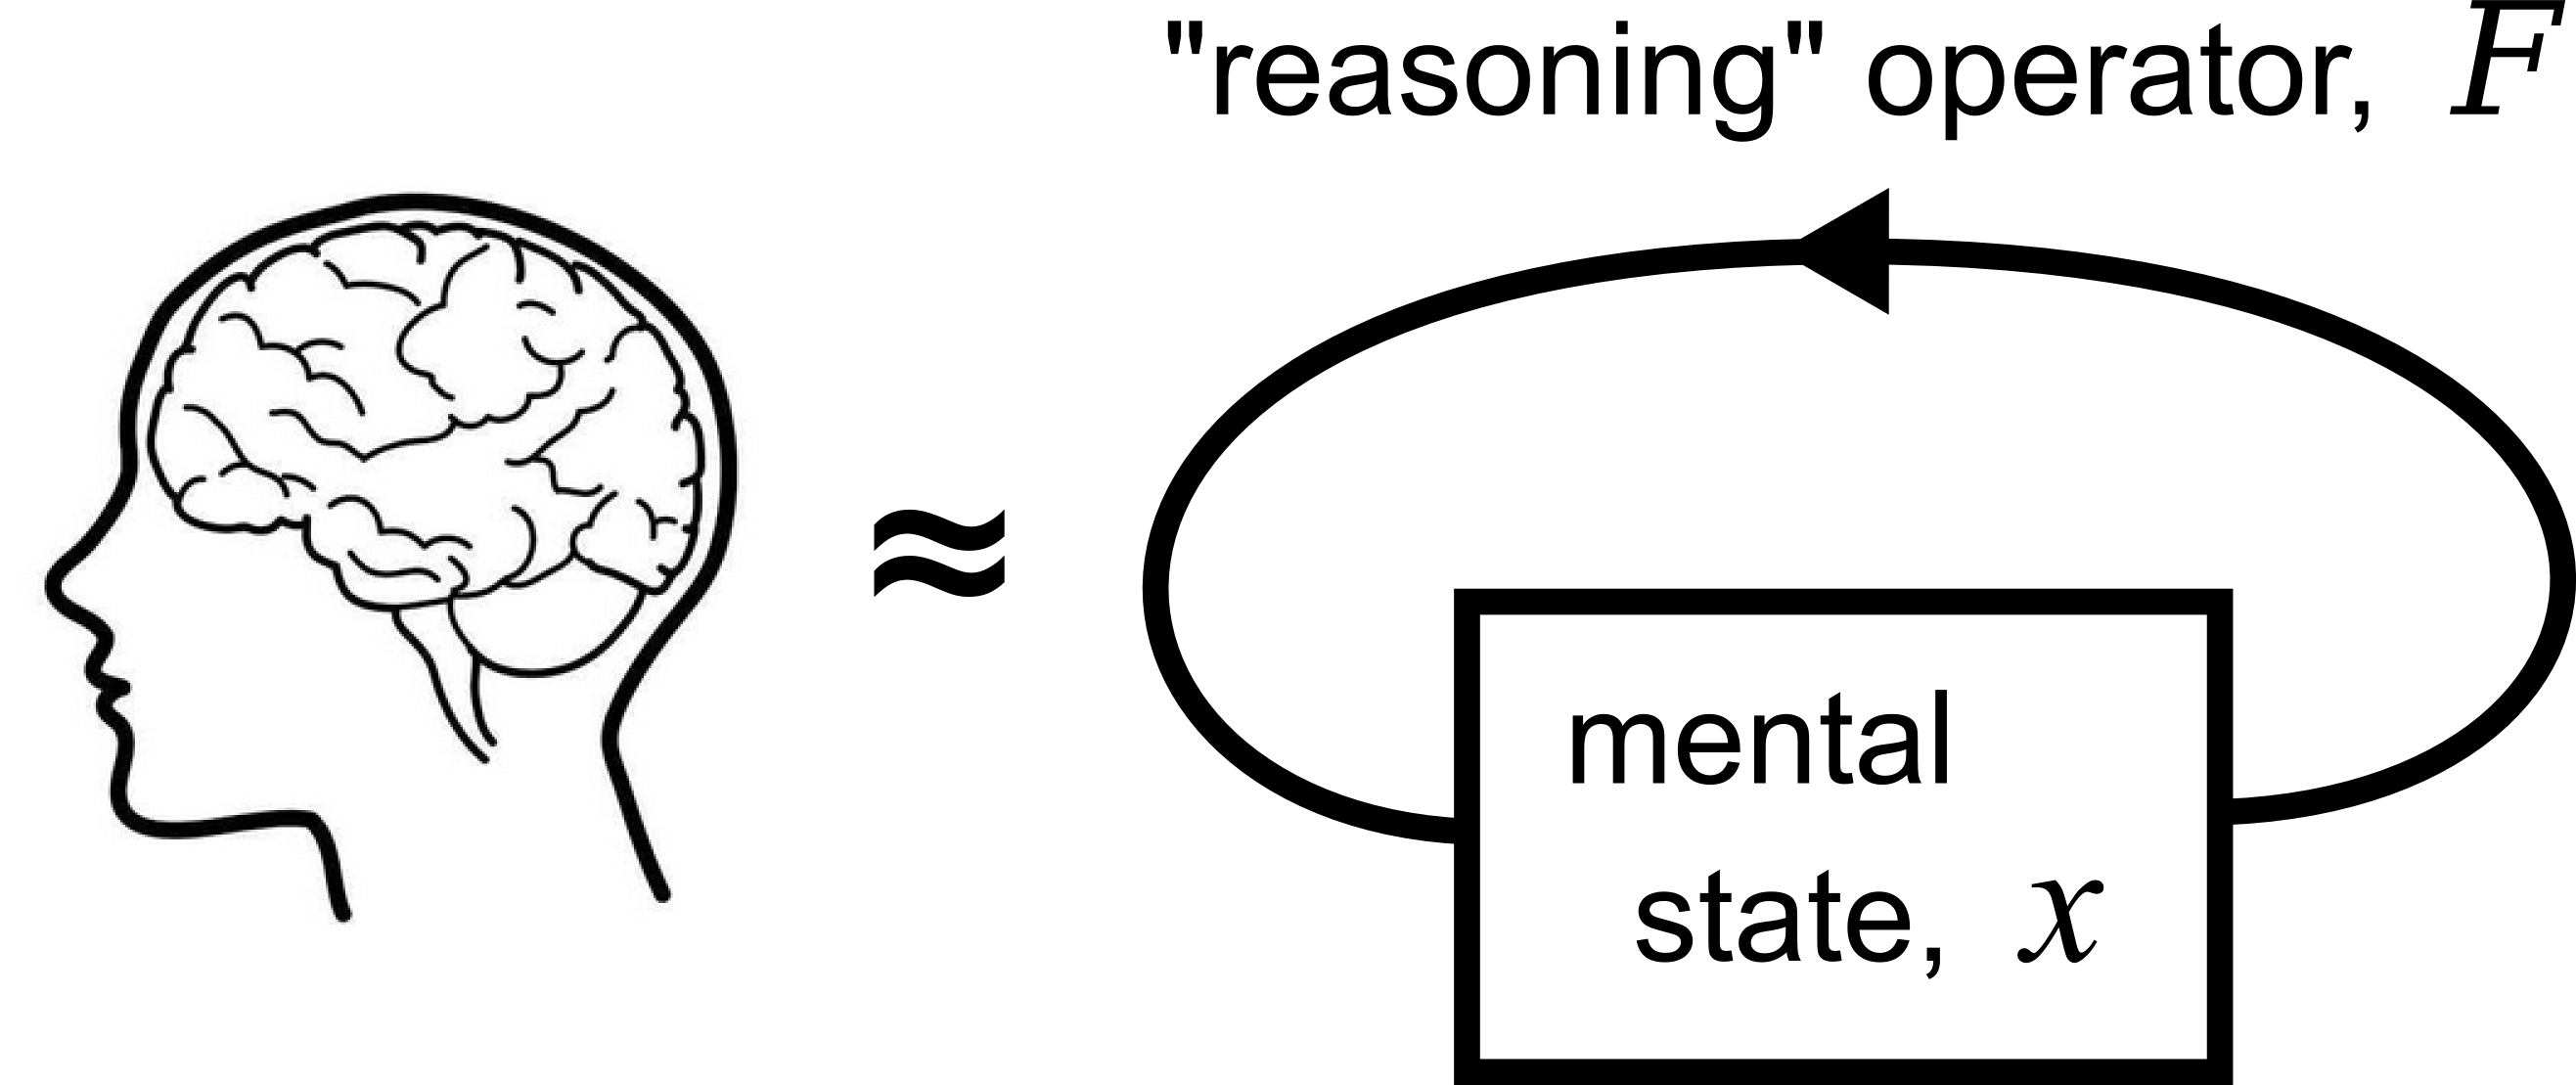
\includegraphics[scale=0.5]{mental-state.png}
\end{equation}

For example, a mental state could be the following set of propositions:
\begin{itemize}
\item I am in my room, writing a paper for AGI-16.
\item I am in the midst of writing the first sentence, ``The main idea is...''
\item I am about to write an infinitive phrase ``to regard...''
\end{itemize}

Thinking is the process of \textbf{transitioning} from one mental state to another.

By representing a cognitive state as a vector $\vec{x} \in X$ where $X$ is the cognitive state-space, the reasoning operator $R$ as a map $X \rightarrow X$, we would have at disposal all the tools available in vector space such as:

\begin{itemize}
\item numerical optimization (including gradient descent)
\item differential equations governing time evolution
\item dynamical systems theory, control theory (eg. adaptive filters)
\item Lie algebra and $C^*$-algebra of continuous operators
\item matrix theory, iteration and fixed-point theory
\item dynamic programming (aka. reinforcement learning)
\item neural networks and deep learning ... etc.
\end{itemize}

This is also partly inspired by the success of Google's PageRank and Word2Vec \cite{} algorithms. %, both exploit the efficiency of vector and matrix calculus.

\section{Relation to Logic-based AI (LBAI)}

In this paper we would jump back and forth between the logic-based view and the dynamical state-space view.

LBAI can be viewed as the compression of a world model into a knowledge-base (KB) of logic formulas:
\begin{equation}
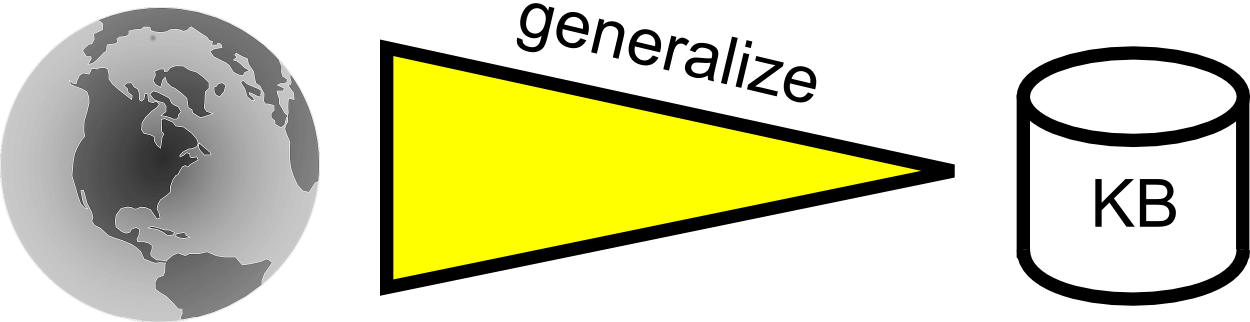
\includegraphics[scale=0.5]{world-model-compression.png}
\end{equation}
The world model is \textit{generated} combinatorially from the set of logic formulas, vaguely reminiscent of a ``basis'' in vector space.  The generative process in logic is much more complicated, contributing to its high \textit{compressive} ability on the one hand, and the \textit{complexity} of learning such formulas on the other hand.

In LBAI the knowledge representation structure is built (\textit{fixed}) from the bottom up:
%\begin{equation}
%\mbox{words } \triangleright \mbox{ sentences } \triangleright \mbox{ logical form } \triangleright \mbox{ logical KB}
%\end{equation}
%Thus the structure of the KB is \textit{fixed} by the human designer. % This rigidity is perhaps why learning in logic-based systems is slow.

% In natural language, an idea can be expressed as a concatenation of words, for example:\\
% And it is just a short jump from word concatenations to symbolic logic.  But this jump may land us into a logic-based ``tar pit'', in which everything is theoretically possible, but often too slow in practice.

%It is just a short jump from the expression of ideas as word concatenations to logical form as linear (or tree-like, or graph-like) compositions of symbols:
\begin{equation}
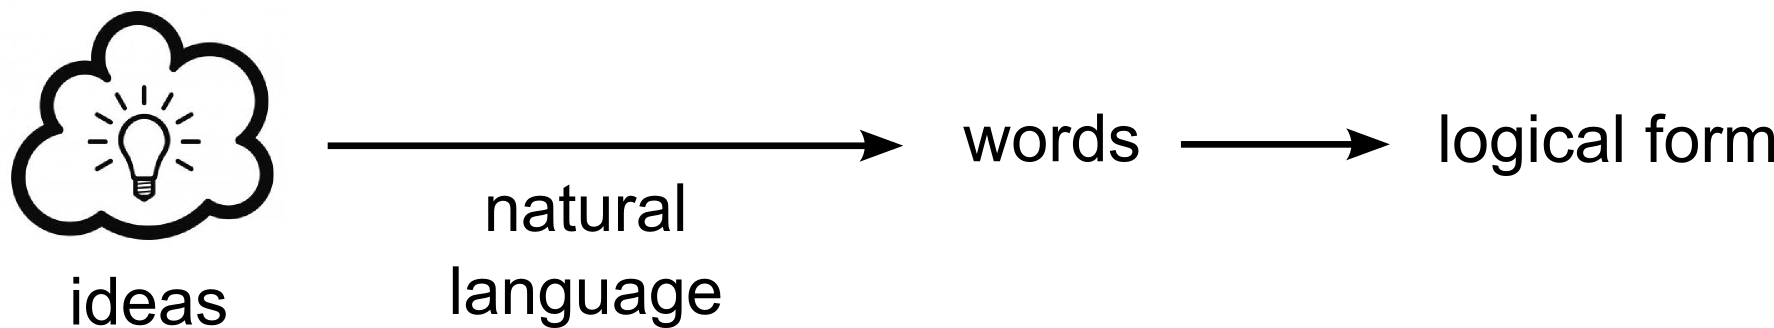
\includegraphics[scale=0.5]{ideas-vs-logical-form.png}
\end{equation}
but is it valid (or profitable) to assume that our mental representations are \textit{isomorphic} to such logical structures?  Or drastically different?

Humans are good at designing symbolic structures, but we don't know how to design \textit{neural} representations which are more or less opaque to us.
Perhaps we could use a neural network acting recurrently on the state vector to \textbf{induce} an internal representation of mental space.  ``\textit{Induced by what},'' you ask?  By the very structure of the neural network itself.  In other words, forcing a neural network to \textit{approximate} the ideal operator $R^*$.

From an abstract point of view, we require:
\begin{itemize}
\item $R$ be an endomorphism: $X \rightarrow X$
\item $R$ has a learning algorithm: $R \stackrel{A}{\longmapsto} R^*$
\end{itemize}

$R$ would contain all the knowledge of the KB, so we expect it to be ``large'' (eg. having a huge number of parameters).  We also desire $R$ to possess a \textbf{hierarchical} structure because hierarchies are computationally very efficient.  A multi-layer perceptron (MLP) seems to be a good candidate, as it is just a bunch of numbers (weight matrices $W$) interleaved by non-linear activation functions:
\begin{equation}
R(\vec{x}) = \sigmoid(W_1 \sigmoid(W_2 ... \sigmoid(W_L \vec{x} )))
\end{equation}
where $L$ is the number of layers.  MLPs would be our starting point to explore more design options.

In 1991 Siegelmann and Sontag \cite{Siegelmann1991} proved that recurrent neural networks (RNNs) can emulate any Turing machine.  In 1993 James Lo \cite{Lo1993} proved that RNNs can universally approximate any non-linear dynamical system.

The idea of $R$ as an operator acting on the state is inspired by the ``consequence operator'' in logic, usually denoted as $\mbox{Cn}$:
\begin{equation}
\mbox{Cn}(\Gamma) = \{ \mbox{ set of propositions that entails from } \Gamma \; \}
\end{equation}
but the function of $R$ can be broader than logical entailment.  We could use $R$ to perform the following functions which are central to LBAI:
\begin{itemize}
\item \textbf{deduction} -- forward- and backward-chaining
\item \textbf{abduction} -- finding explanations
\item \textbf{inductive learning}
\end{itemize}

\begin{tcolorbox}[width=\textwidth,colback={white},title={\centering \textbf{Example 1: } primary-school arithmetic},colbacktitle=white,coltitle=black]

A recurrent neural network is a \textit{much more powerful} learning machine than a feed-forward network, even if they look the same superficially.

\begin{wrapfigure}{l}{2cm}
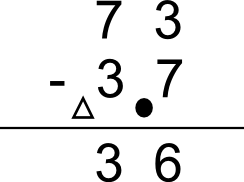
\includegraphics[scale=0.6]{elementary-arithmetic.png}
\end{wrapfigure} 

As an example, consider the way we perform 2-digit subtraction in primary school.  This is done in two steps, and we put a dot on paper to mark ``carry-over''.

The use of the paper is analogous to the ``tape'' in a Turing machine -- the ability to use short-term memory allows us to perform much more complex mental tasks.

We did a simple experiment to train a neural network to perform primary-school subtraction.  The operator is learned easily if we train the two steps \textit{separately}.  The challenge is to find an algorithm that can learn \textbf{multi-step} operations by itself.

\end{tcolorbox}

\begin{tcolorbox}[width=\textwidth,colback={white},title={\centering \textbf{Example 2: } variable binding in predicate logic},colbacktitle=white,coltitle=black]

The following formula in predicate logic defines the ``grandfather'' relation:

\begin{equation}
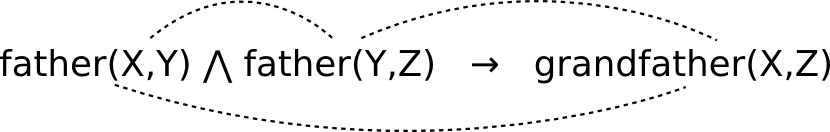
\includegraphics[scale=0.75]{linkage-in-logic-variables.png}
\end{equation}


We did a simple experiment to train a neural network to perform primary-school subtraction.  The operator is learned easily if we train the two steps \textit{separately}.  The challenge is to find an algorithm that can learn \textbf{multi-step} operations by itself.

\end{tcolorbox}  

In LBAI, logic possesses additional structure:
\begin{itemize}
\item \textbf{truth values} (eg. P(rain tomorrow) = 0.7)
\item \textbf{propositional structure} (eg. conjunction: $A \wedge B$) 
\item \textbf{sub-propositional structure} (eg. predication: loves(john, mary) )
\item \textbf{subsumption structure} (eg. $\mbox{dog} \subseteq \mbox{animal}$)
\end{itemize}

These structures can be ``transplanted'' to the vector space $X$ via:
\begin{itemize}
\item \textbf{truth values: } an extra dimension conveying the ``strength'' of states
\item \textbf{propositional structure: } eg. conjunction as vector addition,
\begin{equation}
A \wedge B = \vec{x}_A + \vec{x}_B + ...
\end{equation}
but we have to avoid linear dependencies (``clashing'') such as:
\begin{equation}
\vec{x}_3 = a_1 \vec{x}_1 + a_2 \vec{x}_2
\end{equation}
This would force the vector space dimension to become very high.
\item \textbf{sub-propositional structure: } eg. tensor products as composition of concept atoms:
\begin{equation}
\mbox{loves(john, pete)} = \overrightarrow{john} \otimes \overrightarrow{love} \otimes \overrightarrow{pete}
\end{equation}
\item \textbf{subsumption structure: } eg. define the positive cone $C$ such that
\begin{equation}
\mbox{animal} \supseteq \mbox{dog} \quad \Leftrightarrow \quad \overrightarrow{animal} - \overrightarrow{dog} \in C
\end{equation}
\end{itemize}

But the more logical structure we add to $X$, the more it will resemble logic, and this whole exercise becomes pointless.  Remember our original goal is to try something different from logic, by \textit{relaxing} what defines a logical structure.  So we would selectively add features to $X$.

\section{Misc points}

\begin{itemize}
\item If sigmoid is replaced by polynomial, universal approximating property may be retained.

\item Banach fixed point theorem does not apply because $R$ in general need not be contractive.  Question is whether $R$ necessarily converges to fixed points and the answer is no.

\item If reasoning operator $R$ is continuous, the flow of the dynamical system is governed by an autonomous differential equation.  Poincare-Bendixson only applies to dynamical systems on the plane, and is irrelevant to systems whose phase space has dimension $\geq 3$, or to discrete dynamical systems.

\item Time can be discrete or continuous.

\item Goal is to find minimizer of error (ie, to approximate a function given some input-output data points).  The (finite) set of local minima can be solved via setting $\frac{\partial R}{\partial W} = 0$.  The number of local minima can be calculated as: ?  McClelland paper.

\item If operator is discontinuous, what advantages can be gained?
\end{itemize}

What I want to do now is to determine if $R$ implemented as a deep network is sufficient to model human-level reasoning.

One principle seems to be that logical conclusions must not proliferate indefinitely.  But we are not sure what kind of structural constraints this would impose on the vector space.  Or whether we should impose such constraints manually.

What other properties are desired for the implementation of $R$?

\section{Architecture}

First, cartoon version:
\begin{equation}
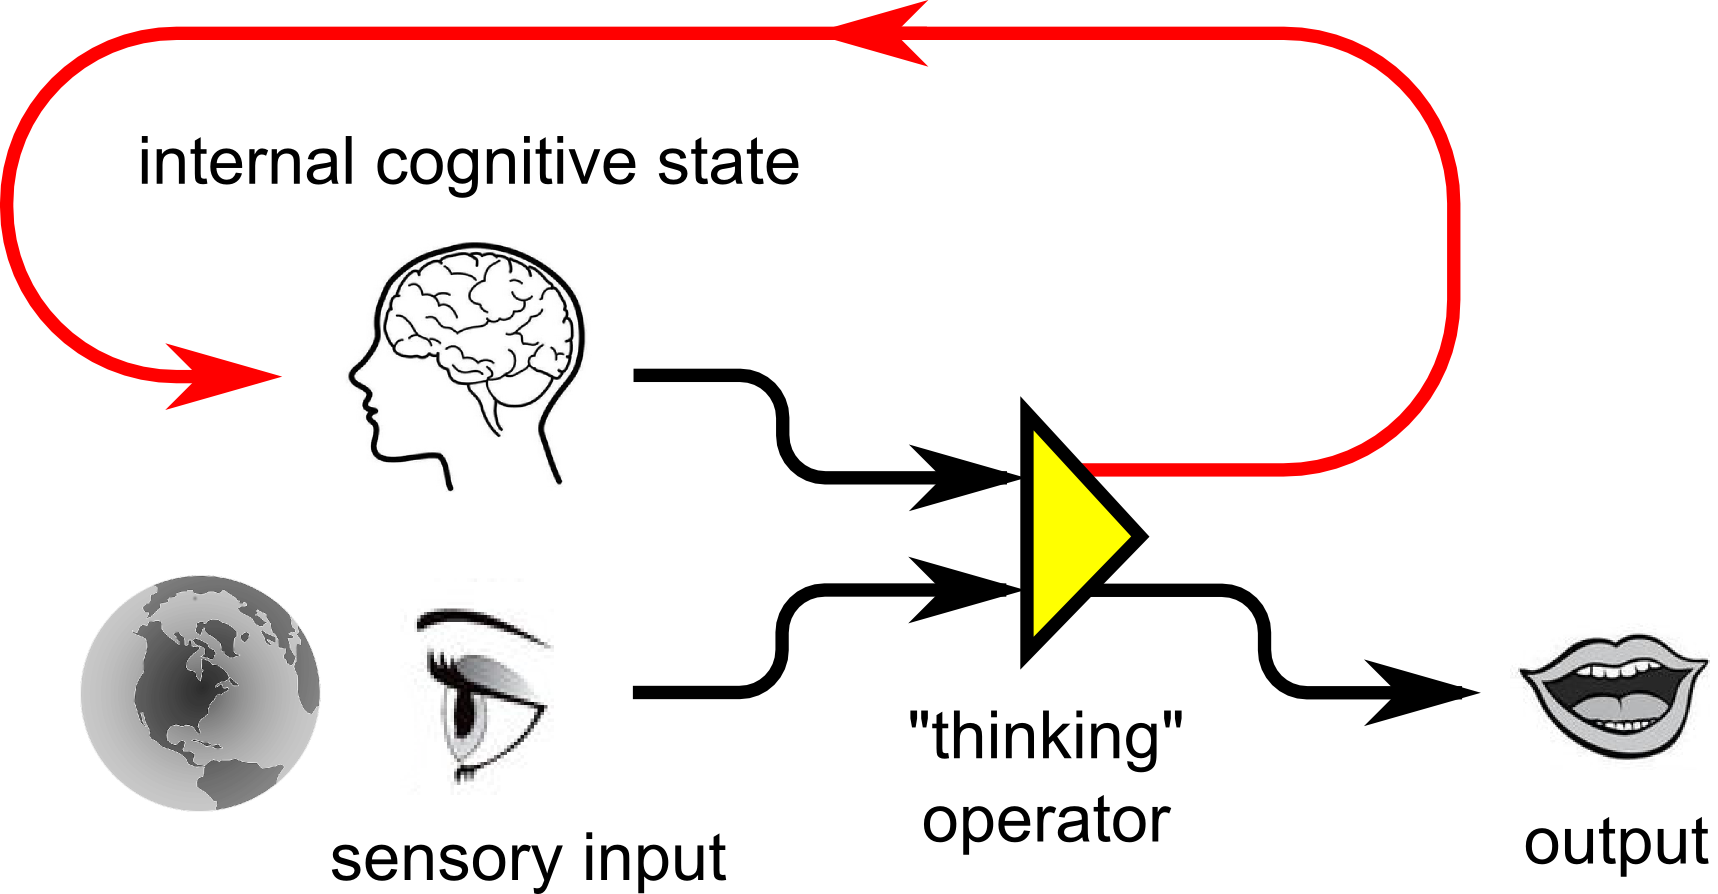
\includegraphics[scale=0.5]{architecture-cartoon.png}
\end{equation}

\begin{equation}
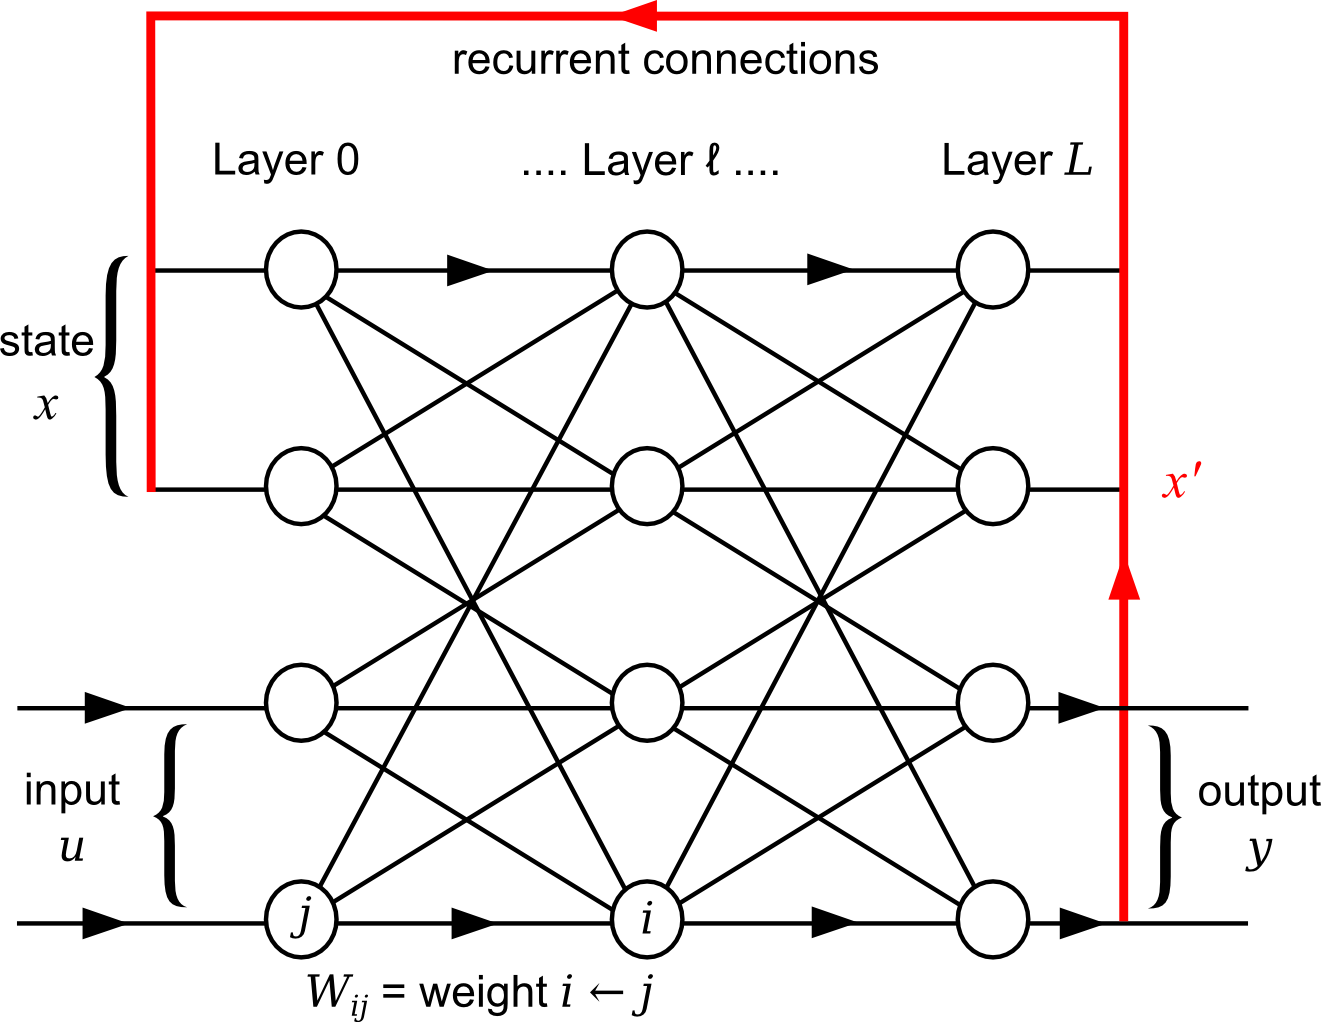
\includegraphics[scale=0.5]{RNN-topology.png}
\end{equation}

TO-DO:  The state space $X$ may be too large and we may need an \textbf{attention mechanism} to select some parts of $X$ for processing by $R$.  This is the notion of \textbf{working memory} in cognitive science.
\begin{equation}
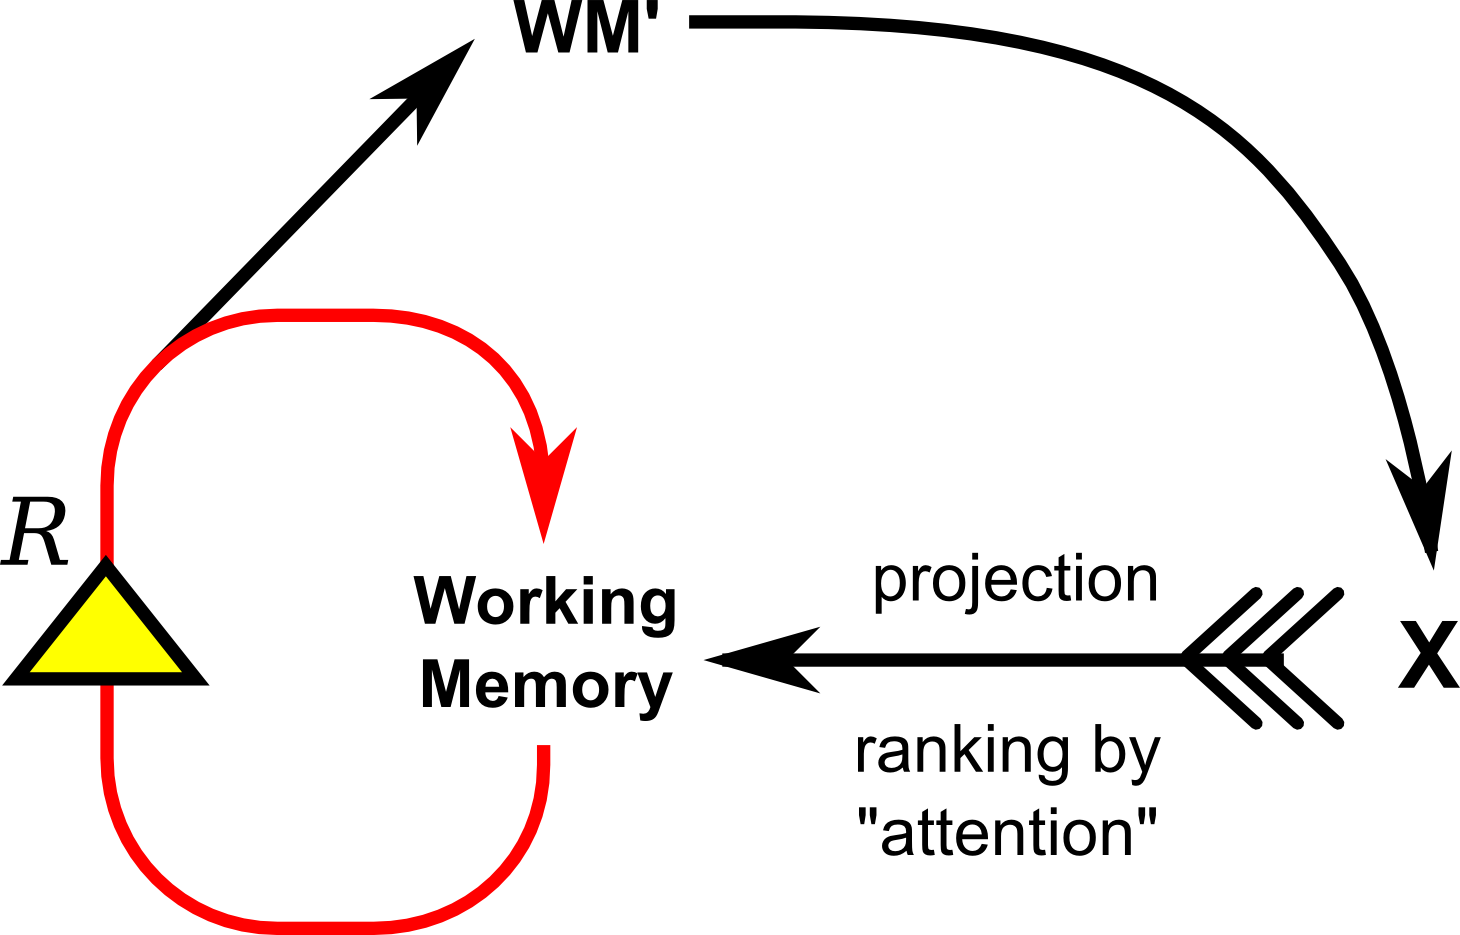
\includegraphics[scale=0.4]{working-memory.png}
\end{equation}

\section{Deep Recurrent Learning}

The learning algorithm for $R$ is central to our system.  $R$ learns to recognize input-output pairs $( \vec{x}_0, \vec{x}^* )$.  What makes it special is that $R$ is allowed to iterate a \textit{flexible} number of times before outputting an answer.  In feed-forward learning we simply learn single-pass recognition, whereas in common recurrent learning we train against a \textit{fixed} time sequence.  Here, the time delay between input and output is allowed to stretch arbitrarily.

Suppose the recurrent network $R$ iterates $n$ times:
\begin{equation}
\vec{x}_{t+1} = \overbrace{R \circ R \circ ...}^{n} (\vec{x})
\end{equation}

As $n \rightarrow \infty$, we get the continuous-time version (a differential equation):
\begin{equation}
\frac{d\vec{x}(t)}{dt} = \mathfrak{R}(\vec{x}(t))
\end{equation}

We could run the network $R$ for a long enough time $T$ such that it is highly likely to reach an equilibrium point.  Then:
\begin{equation}
\vec{x}_{T} = \int_0^T \mathfrak{R}(\vec{x}(t)) dt
\end{equation}
and the error:
\begin{equation}
\mathscr{E} = \vec{x}^* - \vec{x}_{T}
\end{equation}
where $\vec{x}^*$ is the target value which is independent of time.
\begin{eqnarray}
\frac{\partial\mathscr{E}}{\partial\vec{W}} &=& - \frac{\partial}{\partial\vec{W}} \int_0^T \mathfrak{R}(\vec{x}(t)) dt \nonumber \\
&=& - \frac{\partial}{\partial\vec{W}} \int_0^T \sigmoid(W_1 \sigmoid(W_2 ... \sigmoid(W_L \vec{x}(t))) dt
\end{eqnarray}

When there are many layers or if the recurrence is too long, back-prop learning becomes ineffective due to the \textbf{vanishing gradient} problem.  One solution is to use the \textbf{rectifier} activation function:
\begin{equation}
\rectifier (x) = 
\begin{cases}
x, & \mbox{if } x \geq 0 \\
0, & \mbox{otherwise}
\end{cases}
\end{equation}
Since its derivative is piecewise constant, it does not suffer from the vanishing gradient problem.

\subsection{Forward-backward Algorithm}

This is inspired by forward- and backward-chaining in LBAI.  We propagate the state vector from both the initial state $\vec{x}_0$ as well as the final state $\vec{x}^*$.  This bi-directional propagation is added with noise and repeated many times, thus implementing a \textbf{stochastic local search}:

\begin{equation}
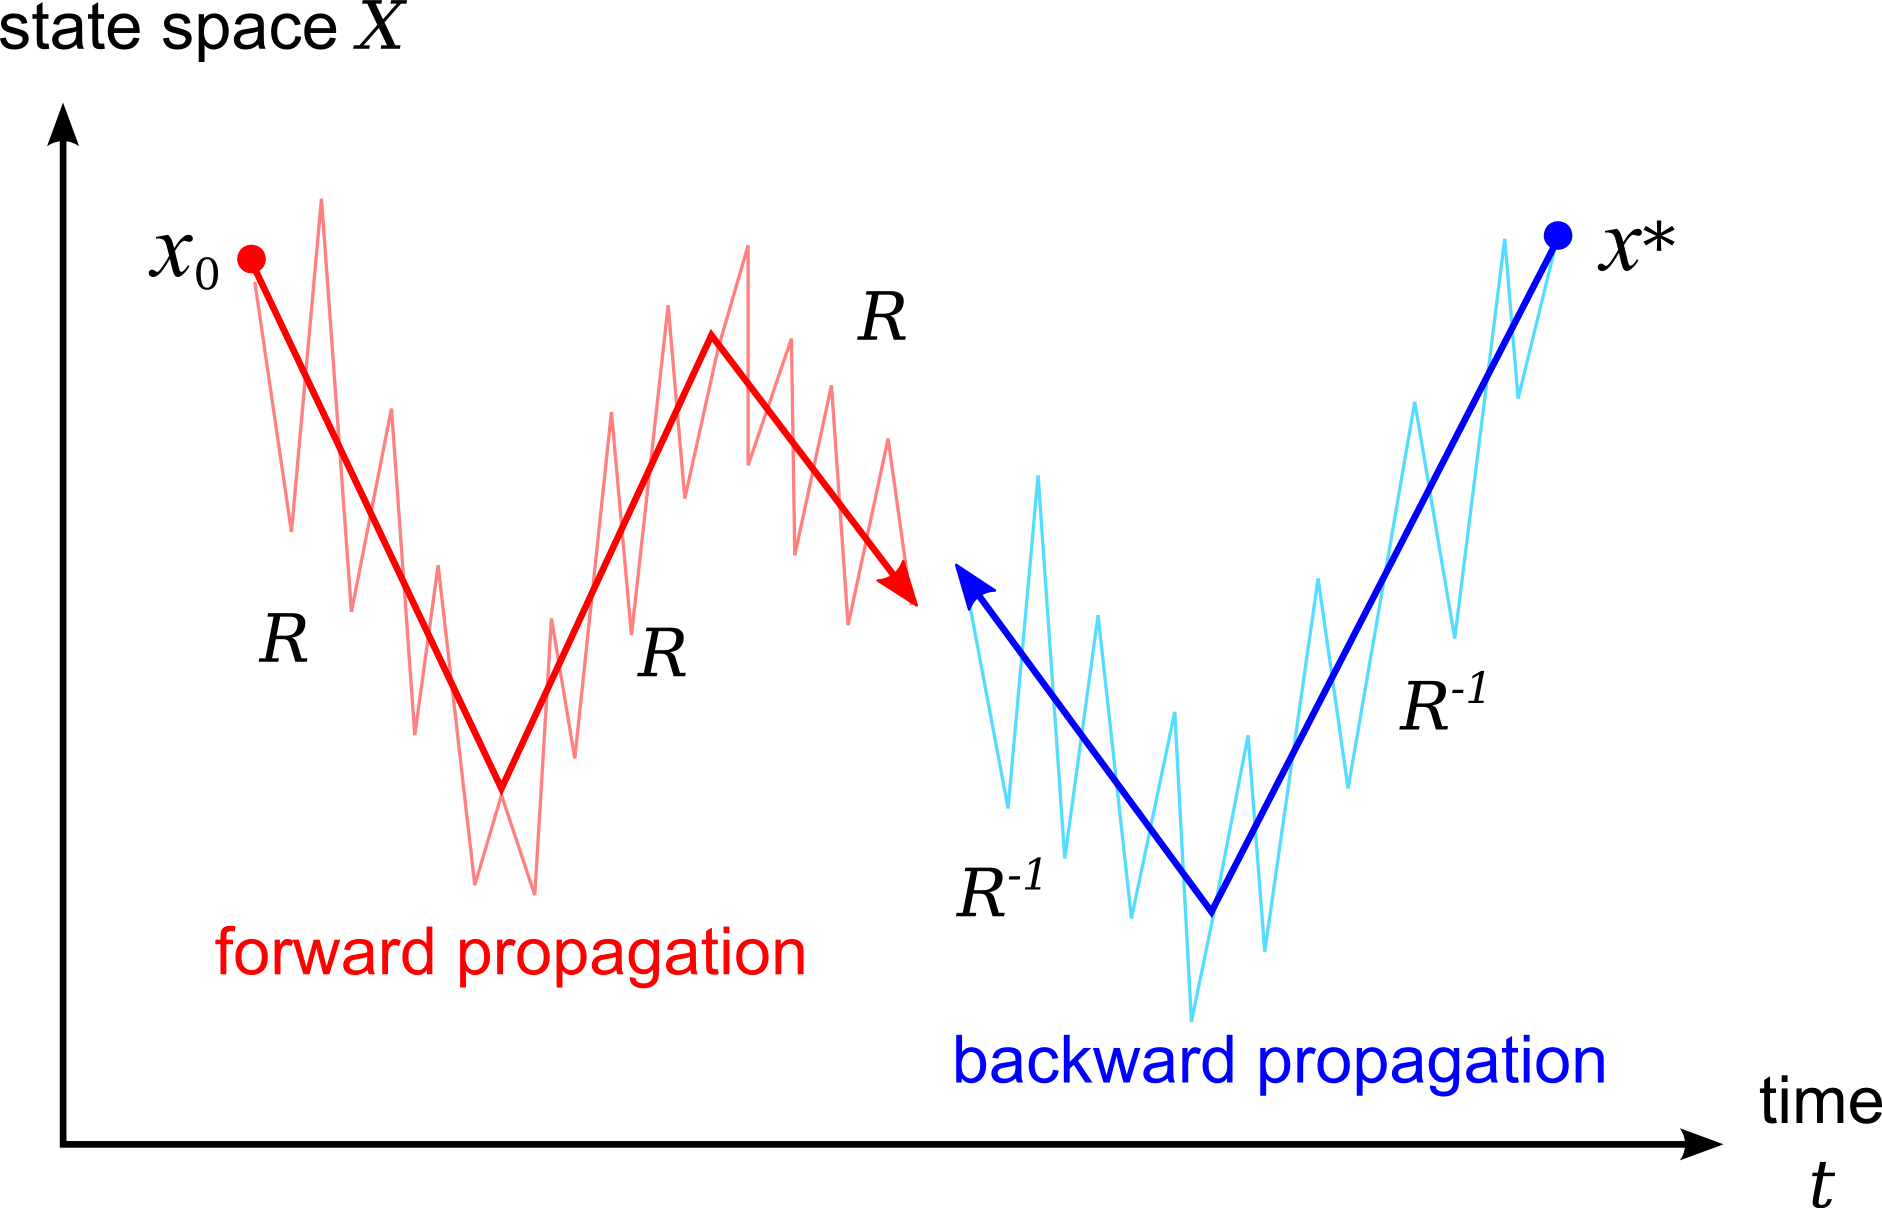
\includegraphics[scale=0.6]{forward-backward-algorithm.png}
\end{equation}

When the forward and backward states get close enough, a successful path is found, and we record the gap and the noises along the path, and use them to train $R$ so that this new path would be recognized.

% One key question is how to deal with "don't care" bits?  One answer is that their errors are zero.  But then this is the same as the error for "correct" weights, which seems not well.  There's got to be a way to alter weights when the answer is correct...

% For \# Iteration = 0, output is immediately known, so potentially the training can be done.  But how to convey that all these alterations of weights are \textbf{optional}?

% \section{Reinforcement learning}

\section*{Acknowledgements}

\footnotesize{In a forum discussion with Ben Goertzel dated 25 June 2014 on the AGI mailing-list: (artificial-general-intelligence @googlegroups.com), YKY asked: Why bother with neural networks, which typically require many neurons to encode data, when logic-based AI can represent a proposition with just a few symbols?  Ben's insight is that neural networks are capable of learning its own representations, and their learning algorithms are relatively fast.  We have been working on "neo-classical" logic-based AI for a long time, and begin to realize that inductive learning in logic (based on combinatorial search in a symbolic space) is perhaps \textit{the bottleneck} in the entire logic-based paradigm.  So we try to look for alternatives that might enable learning to be faster, though we would still emphasize that logic-based AI remains a viable approach to AGI. %, provided that the right search heuristics be found (most probably in the form of \textbf{hierarchical organization} of the learning space).
}

\bibliographystyle{plain} % or number or aaai ...
\bibliography{AGI-book}

\end{document}
